% BHU PYQ -- Professional Exam Template
\documentclass[11pt,a4paper]{article}

\usepackage[a4paper,top=2.5cm,bottom=2.5cm,left=2.8cm,right=2.8cm,headheight=14pt]{geometry}
\usepackage{amsmath,amssymb}
\usepackage[T1]{fontenc}
\usepackage[utf8]{inputenc}
\usepackage{lmodern}
\usepackage{microtype}
\usepackage{fancyhdr}
\usepackage{enumitem}
\usepackage{hyperref}
\usepackage{lastpage}
\usepackage{parskip}
\usepackage{tikz}
\usetikzlibrary{arrows.meta,shapes,positioning,decorations.pathmorphing}

\hypersetup{colorlinks=true,urlcolor=black,linkcolor=black,
  pdftitle={B.Sc. (Hons.) Zoology Sem-III ZOB-301 -- BHU PYQ}}

\pagestyle{fancy}
\fancyhf{}
\renewcommand{\headrulewidth}{0.4pt}
\renewcommand{\footrulewidth}{0.4pt}
\fancyhead[L]{\small   \textit{Banaras Hindu University}}
\fancyhead[R]{\small   \textit{Zoology Paper: ZOB-301}}
\fancyfoot[C]{\small Page  \thepage\ of \pageref{LastPage}}


\newlist{parts}{enumerate}{2}
\setlist[parts,1]{label=(\alph*),leftmargin=*,itemsep=4pt,topsep=3pt}
\setlist[parts,2]{label=(\roman*),leftmargin=*,itemsep=2pt,topsep=2pt}

\newcommand{\pts}[1]{\hfill   \textit{[#1]}}


\begin{document}


\begin{center}
  {\large\bfseries BANARAS HINDU UNIVERSITY}\\[2pt]
  {\normalsize B.Sc. (Hons.) Semester III Examination, 2022-23}\\[6pt]
  \rule{0.8\linewidth}{0.5pt}\\[6pt]
  {\large\bfseries Zoology}\\[4pt]
  {\large\bfseries Paper: ZOB-301 --- Basic Genetics, Evolution and Developmental Biology}\\[4pt]
  {\normalsize Time: Three hours \hfill Full Marks: 70}
\end{center}

\rule{\linewidth}{0.4pt}

\smallskip



\noindent   \textit{Note: Answer three questions from Section-A and three questions from Section-B. Question No. 1 in both sections is compulsory. Use a separate answer book for each section. The figures in the right-hand margin indicate marks.}

\bigskip

\begin{center}
   \textbf{SECTION -- A} \\
   \textbf{(Basic Genetics and Evolution) (Marks: 35)}
\end{center}

\medskip


\noindent   \textbf{Question 1.} Answer the following parts:

\begin{parts}
  \item State whether the following statements are True or False, giving reasons for your answer:\pts{$2  \times 3 = 6$}
  
\begin{parts}
    \item A $t(9;22)$ chromosome translocation is seen in chronic myeloid leukemia.
    \item Polygeny and pleiotropy refer to one and the same phenomenon.
    \item The idea of survival of the fittest was first proposed by Lamarck.
  \end{parts}
  
  \item Define the following terms:\pts{$1  \times 2 = 2$}
  
\begin{parts}
    \item Expressivity
    \item Atavism
  \end{parts}

  \item Select the correct option in each of the following:\pts{$1.5  \times 2 = 3$}
  
\begin{parts}
    \item Which one of the following is not the specific feature of an X-linked recessive pedigree?
    
\begin{enumerate}[label=(\arabic*),leftmargin=*]
      \item Disease affects mainly males.
      \item Affected males have unaffected parents.
      \item Affected males have affected fathers.
      \item Affected males can transmit the disease to their sons.
    \end{enumerate}
    
    \item Industrial melanism is an example of:
    
\begin{enumerate}[label=(\arabic*),leftmargin=*]
      \item Directional selection
      \item Disruptive selection
      \item Stabilizing selection
      \item Artificial selection
    \end{enumerate}
  \end{parts}
\end{parts}

\medskip


\noindent   \textbf{Question 2.} Answer the following parts:

\begin{parts}
  \item Discuss in detail the mechanism of sex determination in   \textit{Drosophila} and humans.\pts{6}
  \item Using suitable examples, explain the features of codominance and incomplete dominance.\pts{6}
\end{parts}

\medskip


\noindent   \textbf{Question 3.} Answer the following parts:

\begin{parts}
  \item What is Hardy-Weinberg equilibrium? Discuss the various factors that disturb the Hardy-Weinberg equilibrium.\pts{6}
  \item Briefly write about the key concepts of Darwinism and the evolutionary significance of variations.\pts{6}
\end{parts}

\medskip


\noindent   \textbf{Question 4.} Write short notes on any two of the following:\dots\pts{$6  \times 2 = 12$}

\begin{parts}
  \item Origin of life
  \item Genetic drift
  \item Chromosomal theory of inheritance
\end{parts}

\pagebreak

\begin{center}
   \textbf{SECTION -- B} \\
   \textbf{(Developmental Biology) (Marks: 35)}
\end{center}

\medskip


\noindent   \textbf{Question 1.} Answer the following parts:

\begin{parts}
  \item Match the items in Column-I with Column-II:\pts{$1  \times 5 = 5$}
  
  
\begin{center}
  
\begin{tabular}{llp{1cm}ll}
    \hline
    \multicolumn{2}{c}{   \textbf{Column-I}} & & \multicolumn{2}{c}{   \textbf{Column-II}} \\
    \hline
    (i) & Acrosomal reaction & & (1) & Morphogenetic movement \\
    (ii) & Cortical reaction & & (2) &   \textit{Amphioxus} \\
    (iii) & Epiboly & & (3) & Calcium wave \\
    (iv) & Area opaca & & (4) & Hyaluronidase \\
    (v) & Microlecithal egg & & (5) & Chick embryo \\
    \hline
  \end{tabular}
  \end{center}

  \item Define the following terms in one/two sentences each:\pts{$1  \times 3 = 3$}
  
\begin{parts}
    \item Epimorphosis
    \item Delamination
    \item Syncytial blastoderm
  \end{parts}

  \item Fill in the blanks with appropriate words:\pts{$1  \times 2 = 2$}
  
\begin{parts}
    \item The process by which cells become specialized in structure and function is called \makebox[3cm]{\hrulefill}.
    \item Primitive streak is formed during the process of \makebox[3cm]{\hrulefill}.
  \end{parts}
\end{parts}

\medskip


\noindent   \textbf{Question 2.} Answer the following parts:

\begin{parts}
  \item With the help of suitable diagrams, describe the process of spermiogenesis.\pts{6}

  
\begin{center}
  
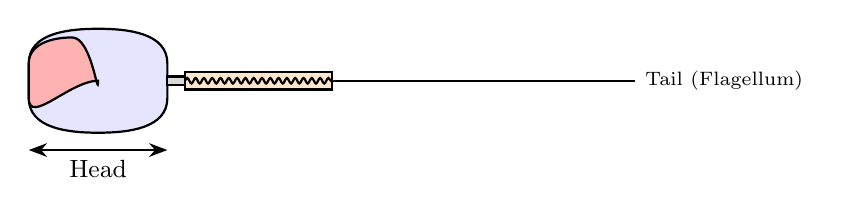
\begin{tikzpicture}[scale=1.1, >=Stealth, every node/.style={font=\small}]
    % Sperm Structure Drawing
    % Head (Acrosome + Nucleus)
    \draw[thick, fill=blue!10!white] (0,0) to[out=90,in=180] (0.8,0.4) to[out=0,in=90] (1.6,0) -- (1.6,-0.4) to[out=270,in=0] (0.8,-0.8) to[out=180,in=270] (0,-0.4) -- cycle;
    \draw[thick, fill=red!30!white] (0,0) to[out=90,in=180] (0.5,0.3) to[out=0,in=270] (0.8,-0.2) to[out=180,in=270] (0,-0.4) -- cycle;
    
ode at (0.4,-0.1) {\scriptsize Acrosome};
    
ode at (1.1,-0.2) {\scriptsize Nucleus};
    
    % Neck / Centriole
    \draw[thick, fill=gray!30!white] (1.6,-0.15) rectangle (1.8,-0.25);
    
ode[above] at (1.7,0.2) {\scriptsize Neck};
    
    % Midpiece (Mitochondria)
    \draw[thick, fill=orange!20!white] (1.8,-0.1) rectangle (3.5,-0.3);
    \draw[thick, decorate, decoration={snake, amplitude=1pt, segment length=3pt}] (1.8,-0.2) -- (3.5,-0.2);
    
ode at (2.65,-0.5) {\scriptsize Midpiece (Mitochondria)};
    
    % Tail (Flagellum)
    \draw[thick] (3.5,-0.2) -- (7.0,-0.2) node[right] {\scriptsize Tail (Flagellum)};

    % Head label
    \draw[thick, <->] (0,-1.0) -- (1.6,-1.0) node[midway, below] {Head};
  \end{tikzpicture}
  \end{center}

  \item What is cleavage? Describe the different types of cleavage on the basis of pattern with suitable examples.\pts{6}
\end{parts}

\pagebreak
\medskip


\noindent   \textbf{Question 3.} Answer the following parts:

\begin{parts}
  \item Give a detailed account of the process of gastrulation in frog with neat and labeled diagrams.\pts{6}

  
\begin{center}
  
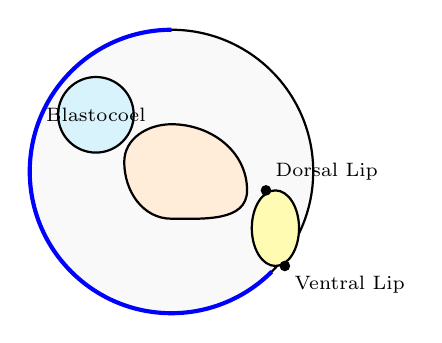
\begin{tikzpicture}[scale=1.2, >=Stealth, every node/.style={font=\small}]
    % Outline of gastrulating embryo
    \draw[thick, fill=gray!5] (0,0) circle (1.5);
    
    % Blastocoel (shrinking cavity at top-left)
    \draw[thick, fill=cyan!15] (-0.8,0.6) circle (0.4) node {\scriptsize Blastocoel};
    
    % Archenteron (growing cavity from right/bottom)
    \draw[thick, fill=orange!15] (0.8,-0.2) to[out=90, in=0] (0,0.5) to[out=180, in=90] (-0.5,0.1) to[out=270, in=180] (0,-0.5) to[out=0, in=270] (0.8,-0.2);
    
ode at (0.2,0.15) {\scriptsize Archenteron};
    
    % Yolk Plug
    \draw[thick, fill=yellow!30!white] (1.1,-0.6) ellipse (0.25 and 0.4);
    
ode[right] at (1.4,-0.6) {\scriptsize Yolk Plug};
    
    % Blastopore Lip (Dorsal and Ventral)
    \draw[fill=black] (1.0,-0.2) circle (0.05) node[above right] {\scriptsize Dorsal Lip};
    \draw[fill=black] (1.2,-1.0) circle (0.05) node[below right] {\scriptsize Ventral Lip};
    
    % Ectoderm (outer layer)
    \draw[line width=1.5pt, blue] (0,1.5) arc (90:315:1.5);
    
ode[left, blue] at (-1.5,0) {\scriptsize Ectoderm};
    
    % Endoderm (yolk cells)
    
ode at (0.2,-0.9) {\scriptsize Endoderm};
  \end{tikzpicture}
  \end{center}

  \item Describe the different morphogenetic movements during gastrulation.\pts{6}
\end{parts}

\medskip


\noindent   \textbf{Question 4.} Write short notes on any two of the following:\pts{$6  \times 2 = 12$}

\begin{parts}
  \item Blastula of chick
  \item Fast block to polyspermy
  \item Regeneration in   \textit{Hydra}
\end{parts}

\vfill
\rule{\linewidth}{0.4pt}

\begin{center}\small
\href{https://bhu-exam.vercel.app/}{Click Here}\\[4pt]\href{https://me-aryan.vercel.app/}{Click Here}\\[4pt]\href{https://quashan-me.vercel.app/}{Click Here}
\end{center}

\end{document}
